\begin{frame}{Diagram equations - Derivation}
    \note<5>{Filename: diagram\_derivation01.tex}

    \emph{Contract $\op{H}_N$ with $\op{T}$ in all possible unique combinations that satisfy a given form. The diagram equation is the sum of all these diagrams.}

    \pause
    \begin{itemize}
        \item Contract one $\op{H}_N$ element with $0,1$ or multiple $\op{T}$ elements. \pause
        \item All $\op{T}$ elements must have \alert{atleast} one contraction with $\op{H}_N$. \pause
        \item No contractions between $\op{T}$ elements are allowed. \pause
        \item A single $\op{T}$ element can contract with a single element of $\op{H}_N$ in different ways.
    \end{itemize}
\end{frame}

\begin{frame}{Diagram elements - Directed lines}
    \note{Filename: diagram\_lines01.tex}

    \begin{figure}
    \centering
        \parbox{0.35\textwidth}{
            \centering
            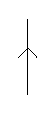
\includegraphics[scale=0.75]{graphics/particleline}
            \caption{Particle line}
        } \qquad
        \parbox{0.35\textwidth}{
            \centering
            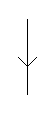
\includegraphics[scale=0.75]{graphics/holeline}
            \caption{Hole line}
        }
    \end{figure}

    \begin{itemize}
        \item Represents a contraction between second quantized operators.
        \item External lines are connected to one operator vertex and infinity.
        \item Internal lines are connected to operator vertices in both ends.
    \end{itemize}

\end{frame}

\begin{frame}{Diagram elements - Onebody Hamiltonian}
    \note{Filename: diagram\_hamiltonian01.tex}

    \renewcommand{\figurename}{Level}

    \begin{figure}
    \centering
    \parbox{0.20\textwidth}{
            \centering
            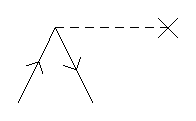
\includegraphics[scale=0.65]{graphics/f1}
            \caption{-1}
        }
        \parbox{0.20\textwidth}{
            \centering
            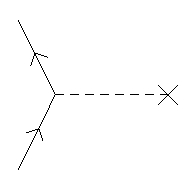
\includegraphics[scale=0.65]{graphics/f2}
            \caption{0}
        }
        \parbox{0.20\textwidth}{
            \centering
            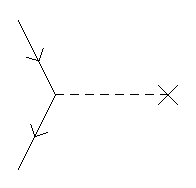
\includegraphics[scale=0.65]{graphics/f3}
            \caption{0}
        }
        \parbox{0.20\textwidth}{
            \centering
            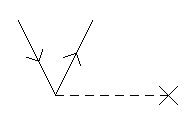
\includegraphics[scale=0.65]{graphics/f4}
            \caption{+1}
        }
    \end{figure}

    \begin{itemize}
        \item Horisontal dashed line segment with one vertex.
        \item Excitation level identify the number of particle/hole pairs created by the operator.
    \end{itemize}
\end{frame}

    
\begin{frame}{Diagram elements - Twobody Hamiltonian}
    \note{Filename: diagram\_hamiltonian02.tex}

    \renewcommand{\figurename}{Level}

    \begin{figure}
    \centering
    \parbox{0.30\textwidth}{
            \centering
            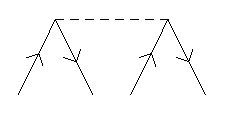
\includegraphics[scale=0.45]{graphics/v1}
            \caption{-2}
        }\quad
        \parbox{0.30\textwidth}{
            \centering
            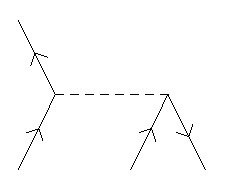
\includegraphics[scale=0.45]{graphics/v2}
            \caption{-1}
        }\quad
        \parbox{0.30\textwidth}{
            \centering
            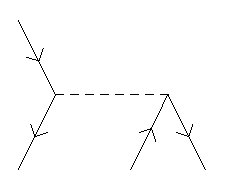
\includegraphics[scale=0.45]{graphics/v3}
            \caption{-1}
        }
    \end{figure}

    \begin{figure}
    \centering
    \parbox{0.30\textwidth}{
            \centering
            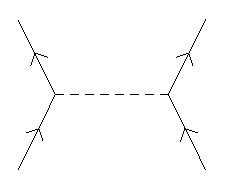
\includegraphics[scale=0.45]{graphics/v4}
            \caption{0}
        }\quad
        \parbox{0.30\textwidth}{
            \centering
            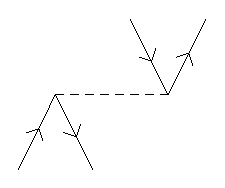
\includegraphics[scale=0.45]{graphics/v5}
            \caption{0}
        }\quad
        \parbox{0.30\textwidth}{
            \centering
            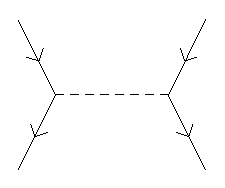
\includegraphics[scale=0.45]{graphics/v6}
            \caption{0}
        }
    \end{figure}

    \begin{figure}
    \centering
    \parbox{0.30\textwidth}{
            \centering
            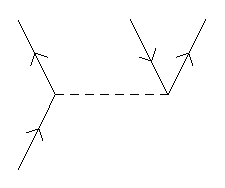
\includegraphics[scale=0.45]{graphics/v7}
            \caption{+1}
        }\quad
        \parbox{0.30\textwidth}{
            \centering
            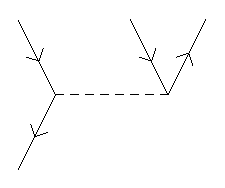
\includegraphics[scale=0.45]{graphics/v8}
            \caption{+1}
        }\quad
        \parbox{0.30\textwidth}{
            \centering
            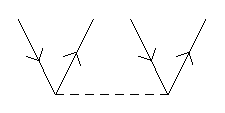
\includegraphics[scale=0.45]{graphics/v9}
            \caption{+2}
        }
    \end{figure}

\end{frame}

\begin{frame}{Diagram elements - Onebody cluster operator}
    \note{Filename: diagram\_cc01.tex}

    \renewcommand{\figurename}{Level}

    \begin{figure}
    \centering
    \parbox{0.20\textwidth}{
            \centering
            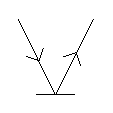
\includegraphics[scale=0.65]{graphics/t1}
            \caption{+1}
        }
    \end{figure}

    \begin{itemize}
        \item Horisontal line segment with one vertex.
        \item Excitation level of +1.
    \end{itemize}
\end{frame}

\begin{frame}{Diagram elements - Twobody cluster operator}
    \note{Filename: diagram\_cc02.tex}

    \renewcommand{\figurename}{Level}

    \begin{figure}
    \centering
    \parbox{0.20\textwidth}{
            \centering
            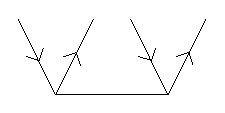
\includegraphics[scale=0.65]{graphics/t2}
            \caption{+2}
        }
    \end{figure}

    \begin{itemize}
        \item Horisontal line segment with two vertices.
        \item Excitation level of +2.
    \end{itemize}
\end{frame}

    
\begin{frame}{CCSD energy equation - Derivation }
    \note{Filename: ccsd\_diagramderivation01.tex}

    \begin{equation*}
        \mathrm{E}_{\mathrm{CCSD}} = \bra{\Phi_0} \barh \ket{\Phi_0}
    \end{equation*}
    \begin{columns}
    \column{0.5\textwidth}
    \begin{itemize}
        \item No external lines.
        \item Final excitation level: 0 
    \end{itemize}
    \column{0.5\textwidth}
    \begin{figure}
        \centering
        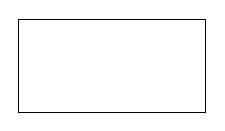
\includegraphics[scale=0.65]{graphics/energy_diag}
    \end{figure}
    \end{columns}
    \renewcommand{\figurename}{Elements}
    \begin{columns}[t]
    \column{0.75\textwidth}
    \begin{figure}
        \caption{$\op{H}_N$}
        \centering
        \parbox{0.20\textwidth}{
            \centering
            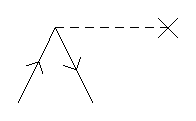
\includegraphics[scale=0.35]{graphics/f1}} 
        \parbox{0.20\textwidth}{
            \centering
            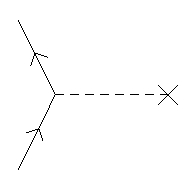
\includegraphics[scale=0.35]{graphics/f2}} 
        \parbox{0.20\textwidth}{
            \centering
            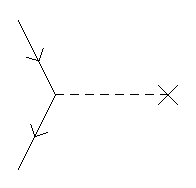
\includegraphics[scale=0.35]{graphics/f3}} 
        \parbox{0.20\textwidth}{
            \centering
            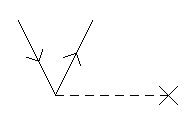
\includegraphics[scale=0.35]{graphics/f4}} 
        \parbox{0.20\textwidth}{
            \centering
            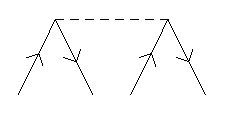
\includegraphics[scale=0.35]{graphics/v1}} 
        \parbox{0.20\textwidth}{
            \centering
            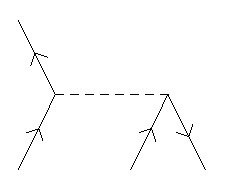
\includegraphics[scale=0.35]{graphics/v2}} 
        \parbox{0.20\textwidth}{
            \centering
            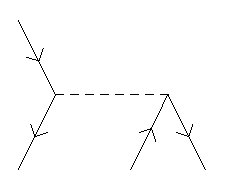
\includegraphics[scale=0.35]{graphics/v3}} 
        \parbox{0.20\textwidth}{
            \centering
            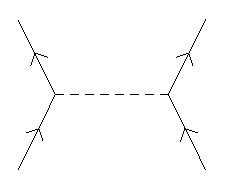
\includegraphics[scale=0.35]{graphics/v4}} 
        \parbox{0.20\textwidth}{
            \centering
            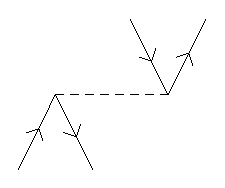
\includegraphics[scale=0.35]{graphics/v5}} 
        \parbox{0.20\textwidth}{
            \centering
            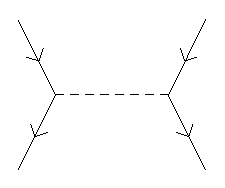
\includegraphics[scale=0.35]{graphics/v6}} 
        \parbox{0.20\textwidth}{
            \centering
            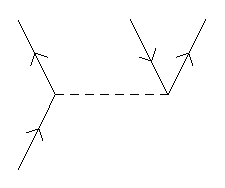
\includegraphics[scale=0.35]{graphics/v7}} 
        \parbox{0.20\textwidth}{
            \centering
            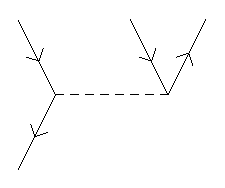
\includegraphics[scale=0.35]{graphics/v8}} 
        \parbox{0.20\textwidth}{
            \centering
            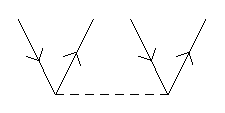
\includegraphics[scale=0.35]{graphics/v9}} 
    \end{figure}
    \column{0.25\textwidth}
    \begin{figure}
        \caption{$\op{T}$}
        \centering
        \parbox[height=3cm]{0.60\textwidth}{
            \centering
            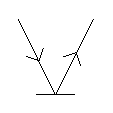
\includegraphics[scale=0.45]{graphics/t1}} 
    \end{figure}
    \begin{figure}
        \parbox[height=3cm]{0.60\textwidth}{
            \centering
            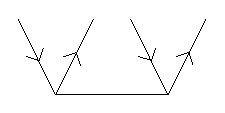
\includegraphics[scale=0.45]{graphics/t2}} 
    \end{figure}
\end{columns}


\end{frame}

\begin{frame}{CCSD energy equation }
    \note{Filename: ccsd\_diagramequations01.tex}
    \begin{equation*}
    E_{CCSD} = 
    \parbox{15mm}{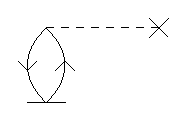
\includegraphics[scale=0.5]{graphics/ccsd_e1}}
    + \parbox{15mm}{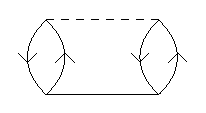
\includegraphics[scale=0.5]{graphics/ccsd_e2}}
    + \parbox{15mm}{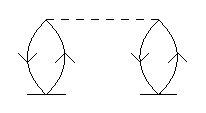
\includegraphics[scale=0.5]{graphics/ccsd_e3}}
\end{equation*}



\end{frame}

\begin{frame}{Diagram rules }
    \note<6>{Filename: diagram\_rules01.tex}

    \begin{itemize}
        \item Label all lines. \pause
        \item Sum over all internal indices. \pause
        \item Extract matrix elements. 
            ($f_{\mathrm{in}}^{\mathrm{out}}$, 
            $\bra{\mathrm{lout, rout}}\ket{\mathrm{lin, rin}}$) \pause
        \item Extract cluster amplitudes with indices in the order left to right. Incoming lines are subscripts, while outgoing lines are superscripts. ($t_{\mathrm{in}}^{\mathrm{out}}$,
                        $t^{\mathrm{lout, rout}}_{\mathrm{lin, rin}}$)\pause
        \item Calculate the phase: $(-1)^{\mathrm{holelines} + \mathrm{loops}}$ \pause
        \item Multiply by a factor of $\frac{1}{2}$ for each equivalent line and each ecuivalent vertex.
    \end{itemize}

\end{frame}

\begin{frame}{CCSD $\op{T}_1$ amplitude equation - Derivation }
    \note{Filename: ccsd\_diagramderivation02.tex}

    \small
    \begin{equation*}
        0 = \bra{\Phi_i^a} \barh \ket{\Phi_0}
    \end{equation*}
    \begin{columns}
    \column{0.5\textwidth}
    \begin{itemize}
        \item One pair of particle/hole  external lines.
        \item Final excitation level: +1
    \end{itemize}
    \column{0.5\textwidth}
    \begin{figure}
        \centering
        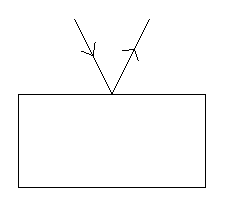
\includegraphics[scale=0.45]{graphics/t1amp_diag}
    \end{figure}
    \end{columns}
    \renewcommand{\figurename}{Elements}
    \begin{columns}[t]
    \column{0.75\textwidth}
    \begin{figure}
        \caption{$\op{H}_N$}
        \centering
        \parbox{0.20\textwidth}{
            \centering
            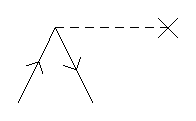
\includegraphics[scale=0.35]{graphics/f1}} 
        \parbox{0.20\textwidth}{
            \centering
            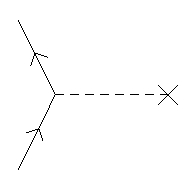
\includegraphics[scale=0.35]{graphics/f2}} 
        \parbox{0.20\textwidth}{
            \centering
            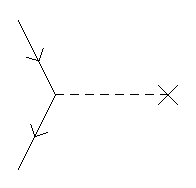
\includegraphics[scale=0.35]{graphics/f3}} 
        \parbox{0.20\textwidth}{
            \centering
            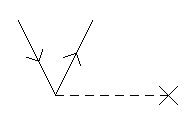
\includegraphics[scale=0.35]{graphics/f4}} 
        \parbox{0.20\textwidth}{
            \centering
            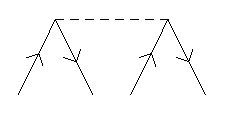
\includegraphics[scale=0.35]{graphics/v1}} 
        \parbox{0.20\textwidth}{
            \centering
            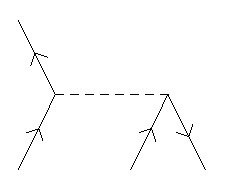
\includegraphics[scale=0.35]{graphics/v2}} 
        \parbox{0.20\textwidth}{
            \centering
            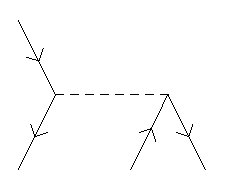
\includegraphics[scale=0.35]{graphics/v3}} 
        \parbox{0.20\textwidth}{
            \centering
            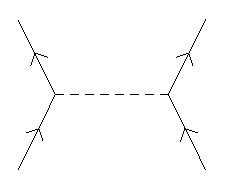
\includegraphics[scale=0.35]{graphics/v4}} 
        \parbox{0.20\textwidth}{
            \centering
            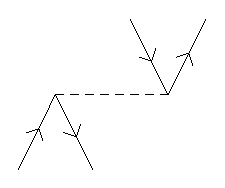
\includegraphics[scale=0.35]{graphics/v5}} 
        \parbox{0.20\textwidth}{
            \centering
            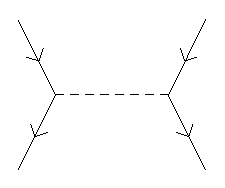
\includegraphics[scale=0.35]{graphics/v6}} 
        \parbox{0.20\textwidth}{
            \centering
            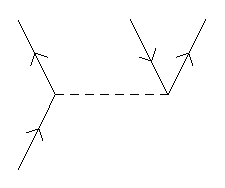
\includegraphics[scale=0.35]{graphics/v7}} 
        \parbox{0.20\textwidth}{
            \centering
            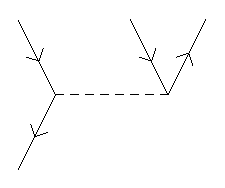
\includegraphics[scale=0.35]{graphics/v8}} 
        \parbox{0.20\textwidth}{
            \centering
            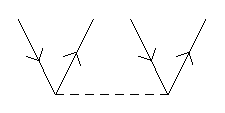
\includegraphics[scale=0.35]{graphics/v9}} 
    \end{figure}
    \column{0.25\textwidth}
    \begin{figure}
        \caption{$\op{T}$}
        \centering
        \parbox[height=3cm]{0.60\textwidth}{
            \centering
            \includegraphics[scale=0.45]{graphics/t1}} 
    \end{figure}
    \begin{figure}
        \parbox[height=3cm]{0.60\textwidth}{
            \centering
            \includegraphics[scale=0.45]{graphics/t2}} 
    \end{figure}
\end{columns}


\end{frame}

    
\begin{frame}{CCSD $\op{T}_1$ amplitude equation }
    \note{Filename: ccsd\_diagramequations02.tex}

\begin{align*}
    0 &= 
    \parbox{10mm}{\includegraphics[scale=0.4]{graphics/ccsd_hbar_04a}}
    + \parbox{18mm}{\includegraphics[scale=0.4]{graphics/ccsd_hbar_04b}}
    + \parbox{15mm}{\includegraphics[scale=0.4]{graphics/ccsd_hbar_04c}}
    + \parbox{15mm}{\includegraphics[scale=0.4]{graphics/ccsd_hbar_04d}} \\
    & \quad + \parbox{21mm}{\includegraphics[scale=0.4]{graphics/ccsd_hbar_04e}}
    + \parbox{17mm}{\includegraphics[scale=0.4]{graphics/ccsd_hbar_04f}}
    + \parbox{15mm}{\includegraphics[scale=0.4]{graphics/ccsd_hbar_04g}}
    + \parbox{15mm}{\includegraphics[scale=0.4]{graphics/ccsd_hbar_04h}} \\
    & \quad + \parbox{17mm}{\includegraphics[scale=0.4]{graphics/ccsd_hbar_04i}}
    + \parbox{15mm}{\includegraphics[scale=0.4]{graphics/ccsd_hbar_04j}}
    + \parbox{20mm}{\includegraphics[scale=0.4]{graphics/ccsd_hbar_04k}}
    + \parbox{15mm}{\includegraphics[scale=0.4]{graphics/ccsd_hbar_04l}} \\
    & \quad + \parbox{17mm}{\includegraphics[scale=0.4]{graphics/ccsd_hbar_04m}}
    + \parbox{15mm}{\includegraphics[scale=0.4]{graphics/ccsd_hbar_04n}}
\end{align*}

\end{frame}

\begin{frame}{Diagram rules }
    \note<6>{Filename: diagram\_rules01.tex}

    \begin{itemize}
        \item Label all lines. \pause
        \item Sum over all internal indices. \pause
        \item Extract matrix elements. 
            ($f_{\mathrm{in}}^{\mathrm{out}}$, 
            $\bra{\mathrm{lout, rout}}\ket{\mathrm{lin, rin}}$) \pause
        \item Extract cluster amplitudes with indices in the order left to right. Incoming lines are subscripts, while outgoing lines are superscripts. ($t_{\mathrm{in}}^{\mathrm{out}}$,
                        $t^{\mathrm{lout, rout}}_{\mathrm{lin, rin}}$)\pause
        \item Calculate the phase: $(-1)^{\mathrm{holelines} + \mathrm{loops}}$ \pause
        \item Multiply by a factor of $\frac{1}{2}$ for each equivalent line and each ecuivalent vertex.
    \end{itemize}

\end{frame}

\begin{frame}{CCSD $\op{T}_1$ amplitude equation }
    \note{Filename: ccsd\_algebraicequations02.tex}

\begin{align*}
    0 &= f_{i}^a + f_{e}^a t_i^e - f_{i}^mt_m^a + \bra{ma}\ket{ei} t_m^e 
        + f_{e}^m t_{im}^{ae} + \frac{1}{2} \bra{am}\ket{ef} t_{im}^{ef} \nn
        &\, - \frac{1}{2} \bra{mn}\ket{ei} t_{mn}^{ea} - f_{e}^m t_i^e t_m^a
        + \bra{am}\ket{ef} t_i^e t_m^f - \bra{mn}\ket{ei} t_m^e t_n^a  \nn
        & \quad + \bra{mn}\ket{ef} t_m^e t_{ni}^{fa}
        - \frac{1}{2} \bra{mn}\ket{ef} t_i^e t_{mn}^{af}
        - \frac{1}{2} \bra{mn}\ket{ef} t_n^a t_{mi}^{ef}\nn
        & \quad  - \bra{mn}\ket{ef} t_i^e t_m^a t_n^f
\end{align*}


\end{frame}

\begin{frame}{CCSD $\op{T}_2$ amplitude equation - Derivation }
    \note{Filename: ccsd\_diagramderivation03.tex}

    \begin{equation*}
        0 = \bra{\Phi_{ij}^{ab}} \barh \ket{\Phi_0}
    \end{equation*}
    \begin{columns}
    \column{0.5\textwidth}
    \begin{itemize}
        \item Two pairs of particle/hole  external lines.
        \item Final excitation level: +2
    \end{itemize}
    \column{0.5\textwidth}
    \begin{figure}
        \centering
        \includegraphics[scale=0.45]{graphics/t2amp_diag}
    \end{figure}
    \end{columns}
    \renewcommand{\figurename}{Elements}
    \begin{columns}[t]
    \column{0.75\textwidth}
    \begin{figure}
        \caption{$\op{H}_N$}
        \centering
        \parbox{0.20\textwidth}{
            \centering
            \includegraphics[scale=0.35]{graphics/f1}} 
        \parbox{0.20\textwidth}{
            \centering
            \includegraphics[scale=0.35]{graphics/f2}} 
        \parbox{0.20\textwidth}{
            \centering
            \includegraphics[scale=0.35]{graphics/f3}} 
        \parbox{0.20\textwidth}{
            \centering
            \includegraphics[scale=0.35]{graphics/f4}} 
        \parbox{0.20\textwidth}{
            \centering
            \includegraphics[scale=0.35]{graphics/v1}} 
        \parbox{0.20\textwidth}{
            \centering
            \includegraphics[scale=0.35]{graphics/v2}} 
        \parbox{0.20\textwidth}{
            \centering
            \includegraphics[scale=0.35]{graphics/v3}} 
        \parbox{0.20\textwidth}{
            \centering
            \includegraphics[scale=0.35]{graphics/v4}} 
        \parbox{0.20\textwidth}{
            \centering
            \includegraphics[scale=0.35]{graphics/v5}} 
        \parbox{0.20\textwidth}{
            \centering
            \includegraphics[scale=0.35]{graphics/v6}} 
        \parbox{0.20\textwidth}{
            \centering
            \includegraphics[scale=0.35]{graphics/v7}} 
        \parbox{0.20\textwidth}{
            \centering
            \includegraphics[scale=0.35]{graphics/v8}} 
        \parbox{0.20\textwidth}{
            \centering
            \includegraphics[scale=0.35]{graphics/v9}} 
    \end{figure}
    \column{0.25\textwidth}
    \begin{figure}
        \caption{$\op{T}$}
        \centering
        \parbox[height=3cm]{0.60\textwidth}{
            \centering
            \includegraphics[scale=0.45]{graphics/t1}} 
    \end{figure}
    \begin{figure}
        \parbox[height=3cm]{0.60\textwidth}{
            \centering
            \includegraphics[scale=0.45]{graphics/t2}} 
    \end{figure}
\end{columns}


\end{frame}

\begin{frame}{CCSD $\op{T}_2$ amplitude equation }
    \note{Filename: ccsd\_diagramequations03.tex}

\begin{align*}
    0 &= 
    \parbox{10mm}{\includegraphics[scale=0.25]{graphics/ccsd_hbar_13_01}} + 
    \parbox{10mm}{\includegraphics[scale=0.25]{graphics/ccsd_hbar_13_02}} + 
    \parbox{10mm}{\includegraphics[scale=0.25]{graphics/ccsd_hbar_13_03}} +
    \parbox{14mm}{\includegraphics[scale=0.25]{graphics/ccsd_hbar_13_04}} + 
    \parbox{14mm}{\includegraphics[scale=0.25]{graphics/ccsd_hbar_13_05}} + 
    \parbox{14mm}{\includegraphics[scale=0.25]{graphics/ccsd_hbar_13_06}} \nn
    & + \parbox{14mm}{\includegraphics[scale=0.25]{graphics/ccsd_hbar_13_07}} + 
    \parbox{14mm}{\includegraphics[scale=0.25]{graphics/ccsd_hbar_13_08}} + 
    \parbox{14mm}{\includegraphics[scale=0.25]{graphics/ccsd_hbar_13_09}} +
    \parbox{14mm}{\includegraphics[scale=0.25]{graphics/ccsd_hbar_13_10}} + 
    \parbox{14mm}{\includegraphics[scale=0.25]{graphics/ccsd_hbar_13_11}} \nn
    & + \parbox{15mm}{\includegraphics[scale=0.25]{graphics/ccsd_hbar_13_12}} +
    \parbox{19mm}{\includegraphics[scale=0.25]{graphics/ccsd_hbar_13_13}} + 
    \parbox{15mm}{\includegraphics[scale=0.25]{graphics/ccsd_hbar_13_14}} +
    \parbox{15mm}{\includegraphics[scale=0.25]{graphics/ccsd_hbar_13_15}} + 
    \parbox{15mm}{\includegraphics[scale=0.25]{graphics/ccsd_hbar_13_16}} \nn
    & + \parbox{15mm}{\includegraphics[scale=0.25]{graphics/ccsd_hbar_13_17}} +
    \parbox{17mm}{\includegraphics[scale=0.25]{graphics/ccsd_hbar_13_18}} + 
    \parbox{15mm}{\includegraphics[scale=0.25]{graphics/ccsd_hbar_13_19}} +
    \parbox{15mm}{\includegraphics[scale=0.25]{graphics/ccsd_hbar_13_20}} + 
    \parbox{15mm}{\includegraphics[scale=0.25]{graphics/ccsd_hbar_13_21}} \nn
    & + \parbox{15mm}{\includegraphics[scale=0.25]{graphics/ccsd_hbar_13_22}} + 
    \parbox{15mm}{\includegraphics[scale=0.25]{graphics/ccsd_hbar_13_23}} +
    \parbox{15mm}{\includegraphics[scale=0.25]{graphics/ccsd_hbar_13_24}} + 
    \parbox{15mm}{\includegraphics[scale=0.25]{graphics/ccsd_hbar_13_25}} +
    \parbox{15mm}{\includegraphics[scale=0.25]{graphics/ccsd_hbar_13_26}} \nn
    & + \parbox{16mm}{\includegraphics[scale=0.25]{graphics/ccsd_hbar_13_27}} +
    \parbox{17mm}{\includegraphics[scale=0.25]{graphics/ccsd_hbar_13_28}} + 
    \parbox{14mm}{\includegraphics[scale=0.25]{graphics/ccsd_hbar_13_29}} +
    \parbox{15mm}{\includegraphics[scale=0.25]{graphics/ccsd_hbar_13_30}} + 
    \parbox{15mm}{\includegraphics[scale=0.25]{graphics/ccsd_hbar_13_31}}
\end{align*}

\end{frame}

\begin{frame}{Diagram rules }
    \note<7>{Filename: diagram\_rules02.tex}

    \begin{itemize}
        \item Label all lines. \pause
        \item Sum over all internal indices. \pause
        \item Extract matrix elements. 
            ($f_{\mathrm{in}}^{\mathrm{out}}$, 
            $\bra{\mathrm{lout, rout}}\ket{\mathrm{lin, rin}}$) \pause
        \item Extract cluster amplitudes with indices in the order left to right. Incoming lines are subscripts, while outgoing lines are superscripts. ($t_{\mathrm{in}}^{\mathrm{out}}$,
                        $t^{\mathrm{lout, rout}}_{\mathrm{lin, rin}}$)\pause
        \item Calculate the phase: $(-1)^{\mathrm{holelines} + \mathrm{loops}}$ \pause
        \item Multiply by a factor of $\frac{1}{2}$ for each equivalent line and each ecuivalent vertex. \pause
        \item Antisymmetrize a pair of external particle/hole line that does not connect to the same operator.
    \end{itemize}

\end{frame}

\begin{frame}{CCSD $\op{T}_2$ amplitude equation }
    \note{Filename: ccsd\_algebraicequations03.tex}
    \scriptsize
\begin{align*}
    0 &= 
        \bra{ab} \ket{ij}
        + P(ij) \bra{ab}\ket{ej} t_i^e
        - P(ab) \bra{am} \ket{ij} t_m^b
        + P(ab) f_{e}^b t_{ij}^{ae}
        - P(ij) f_{i}^m t_{mj}^{ab} \nn
        & + \, \frac{1}{2} \bra{ab}\ket{ef} t_{ij}^{ef}
        + \frac{1}{2} \bra{mn}\ket{ij} t_{mn}^{ab}
        + P(ij) P(ab) \bra{mb}\ket{ej} t_{im}^{ae} \nn
        & + \, \frac{1}{2} P(ij) \bra{ab}\ket{ef} t_i^e t_j^f
        + \frac{1}{2} P(ab) \bra{mn}\ket{ij} t_m^a t_n^b
        - P(ij) P(ab) \bra{mb}\ket{ej} t_i^e t_m^a \nn
        & + \, \frac{1}{4} \bra{mn}\ket{ef} t_{ij}^{ef} t_{mn}^{ab}
        + \frac{1}{2} P(ij) P(ab) \bra{mn}\ket{ef} t_{im}^{ae} t_{nj}^{fb}
        - \frac{1}{2} P(ab) \bra{mn}\ket{ef} t_{ij}^{ae} t_{mn}^{bf} \nn
        & - \, \frac{1}{2} P(ij) \bra{mn}\ket{ef} t_{mi}^{ef} t_{nj}^{ab}
        - P(ij) f_{e}^m t_i^e t_{mj}^{ab}
        - P(ab) f_{e}^m t_{ij}^{ae} t_m^b \nn
        & + \, P(ij) P(ab) \bra{am}\ket{ef} t_i^e t_{mj}^{fb}
        - \frac{1}{2} P(ab) \bra{am}\ket{ef} t_{ij}^{ef} t_m^b
        + P(ab) \bra{bm}\ket{ef} t_{ij}^{ae} t_m^f \nn
        & - \, P(ij) P(ab) \bra{mn} \ket{ej} t_{im}^{ae} t_n^b
        + \frac{1}{2} P(ij) \bra{mn}\ket{ej} t_i^e t_{mn}^{ab}
        -P(ij) \bra{mn}\ket{ei} t_m^e t_{nj}^{ab} \nn
        & - \, \frac{1}{2} P(ij) P(ab) \bra{am}\ket{ef} t_i^e t_j^f t_m^b
        + \frac{1}{2} P(ij) P(ab) \bra{mn}\ket{ej} t_i^e t_m^a t_n^b \nn
        & + \, \frac{1}{4} P(ij) \bra{mn}\ket{ef} t_i^e t_{mn}^{ab} t_j^f
        - P(ij) P(ab) \bra{mn}\ket{ef} t_i^e t_m^a t_{nj}^{fb} \nn
        & + \, \frac{1}{4} P(ab) \bra{mn}\ket{ef} t_m^a t_{ij}^{ef} t_n^b
        - P(ij) \bra{mn}\ket{ef} t_m^e t_i^f t_{nj}^{ab}
        - P(ab) \bra{mn}\ket{ef} t_{ij}^{ae} t_m^b t_n^f \nn
        & + \, \frac{1}{4} P(ij) P(ab) \bra{mn}\ket{ef} t_i^e t_m^a t_j^f t_n^b \nn
\end{align*}

\end{frame}

